\begin{figure}[h] 
\centering 
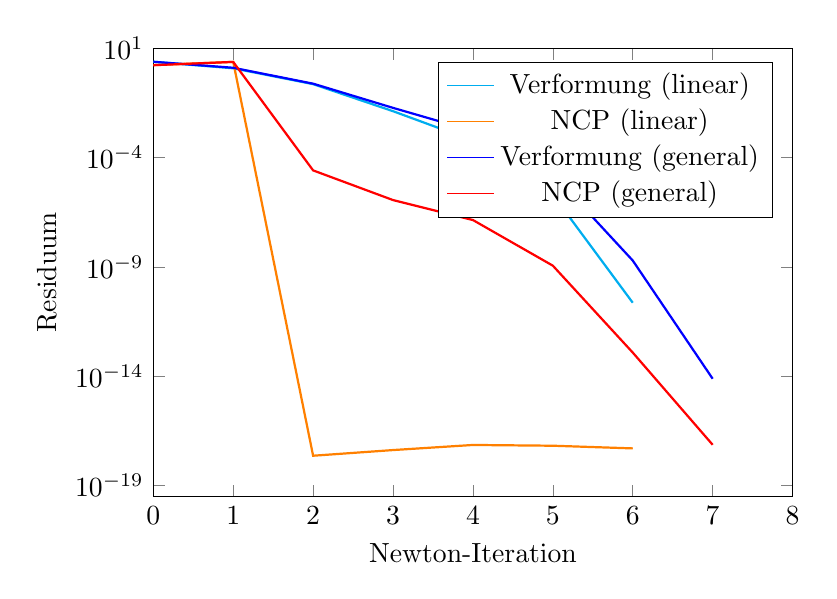
\begin{tikzpicture}[every plot/.append style={thick}] 
\begin{axis}[ 
label style={font=\normalsize}, 
xlabel={Newton-Iteration}, 
ylabel={Residuum}, 
xmin=0, xmax=8, 
ymode=log, 
ymin=0, ymax=10, 
width=0.8\textwidth, 
height=0.6\textwidth, 
legend pos=north east, 
legend style={cells={align=left}}, 
grid style=dashed, 
] 
\addplot[ 
color=cyan, 
] 
coordinates { 
(0, 2.39e+00)(1, 1.20e+00)(2, 2.26e-01)(3, 1.31e-02)(4, 5.93e-04)(5, 1.99e-06)(6, 2.28e-11)}; 
\addlegendentry{Verformung (linear)} 
\addplot[ 
color=orange, 
] 
coordinates { 
(0, 1.68e+00)(1, 2.36e+00)(2, 2.30e-18)(3, 4.18e-18)(4, 7.15e-18)(5, 6.60e-18)(6, 4.98e-18)}; 
\addlegendentry{NCP (linear)} 
\addplot[ 
color=blue, 
] 
coordinates { 
(0, 2.39e+00)(1, 1.27e+00)(2, 2.38e-01)(3, 1.86e-02)(4, 1.63e-03)(5, 1.73e-05)(6, 1.94e-09)(7, 7.64e-15)}; 
\addlegendentry{Verformung (general)} 
\addplot[ 
color=red, 
] 
coordinates { 
(0, 1.66e+00)(1, 2.35e+00)(2, 2.57e-05)(3, 1.13e-06)(4, 1.38e-07)(5, 1.13e-09)(6, 1.20e-13)(7, 7.28e-18)}; 
\addlegendentry{NCP (general)} 
\end{axis} 
\end{tikzpicture} 
\caption{Residuen des Stoffgesetzes 'St.Venant' mit Hinderniss 'Parabel' und 162 Freiheitsgraden für die Verschiebung.} 
\label{fiq:St.Venant_Parabel_level2} 
\end{figure} 
